\indent\underline{\textbf{Ejercicio 4}}\\
En el Ejemplo 4.3 (\textit{Gambler’s problem, Sutton\&Barto, 2018})~\cite{Sutton2018}, la política óptima tiene una forma particular (ver figura~\ref{fig:gamblers_problem}) con máximo en $50$.
Es decir, cuando el jugador tiene $\$50$, le conviene apostarlo todo; sin embargo, cuando tiene $\$51$, le
conviene apostar $\$1$.
¿Por qué sucede esto?

\begin{figure}[H]
    \centering
    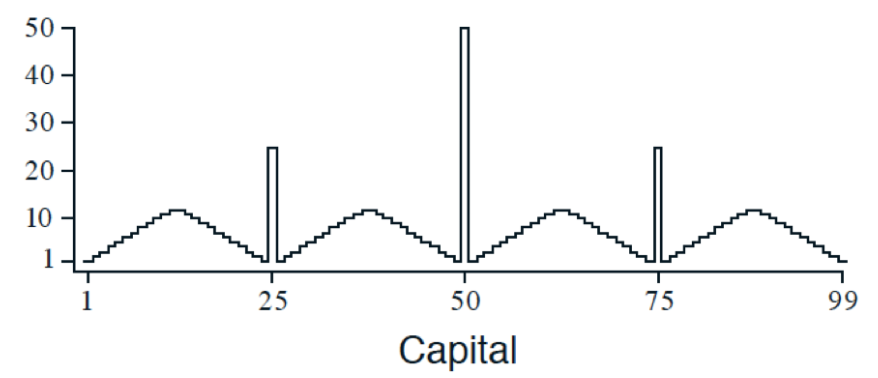
\includegraphics[width=0.5\textwidth]{../img/gamblers_problem}
    \caption{Ejemplo 4.3, Sutton\&Barto, 2018}\label{fig:gamblers_problem}
\end{figure}

\indent\underline{\textbf{Solución}}\\

\line(1,0){\textwidth}
